\section{Results, Analysis, and Relevant Information}

图片待改

\subsection{Results and Analysis}
\begin{figure}[htbp]
    \centering
    \begin{subfigure}[t]{0.4\linewidth}
        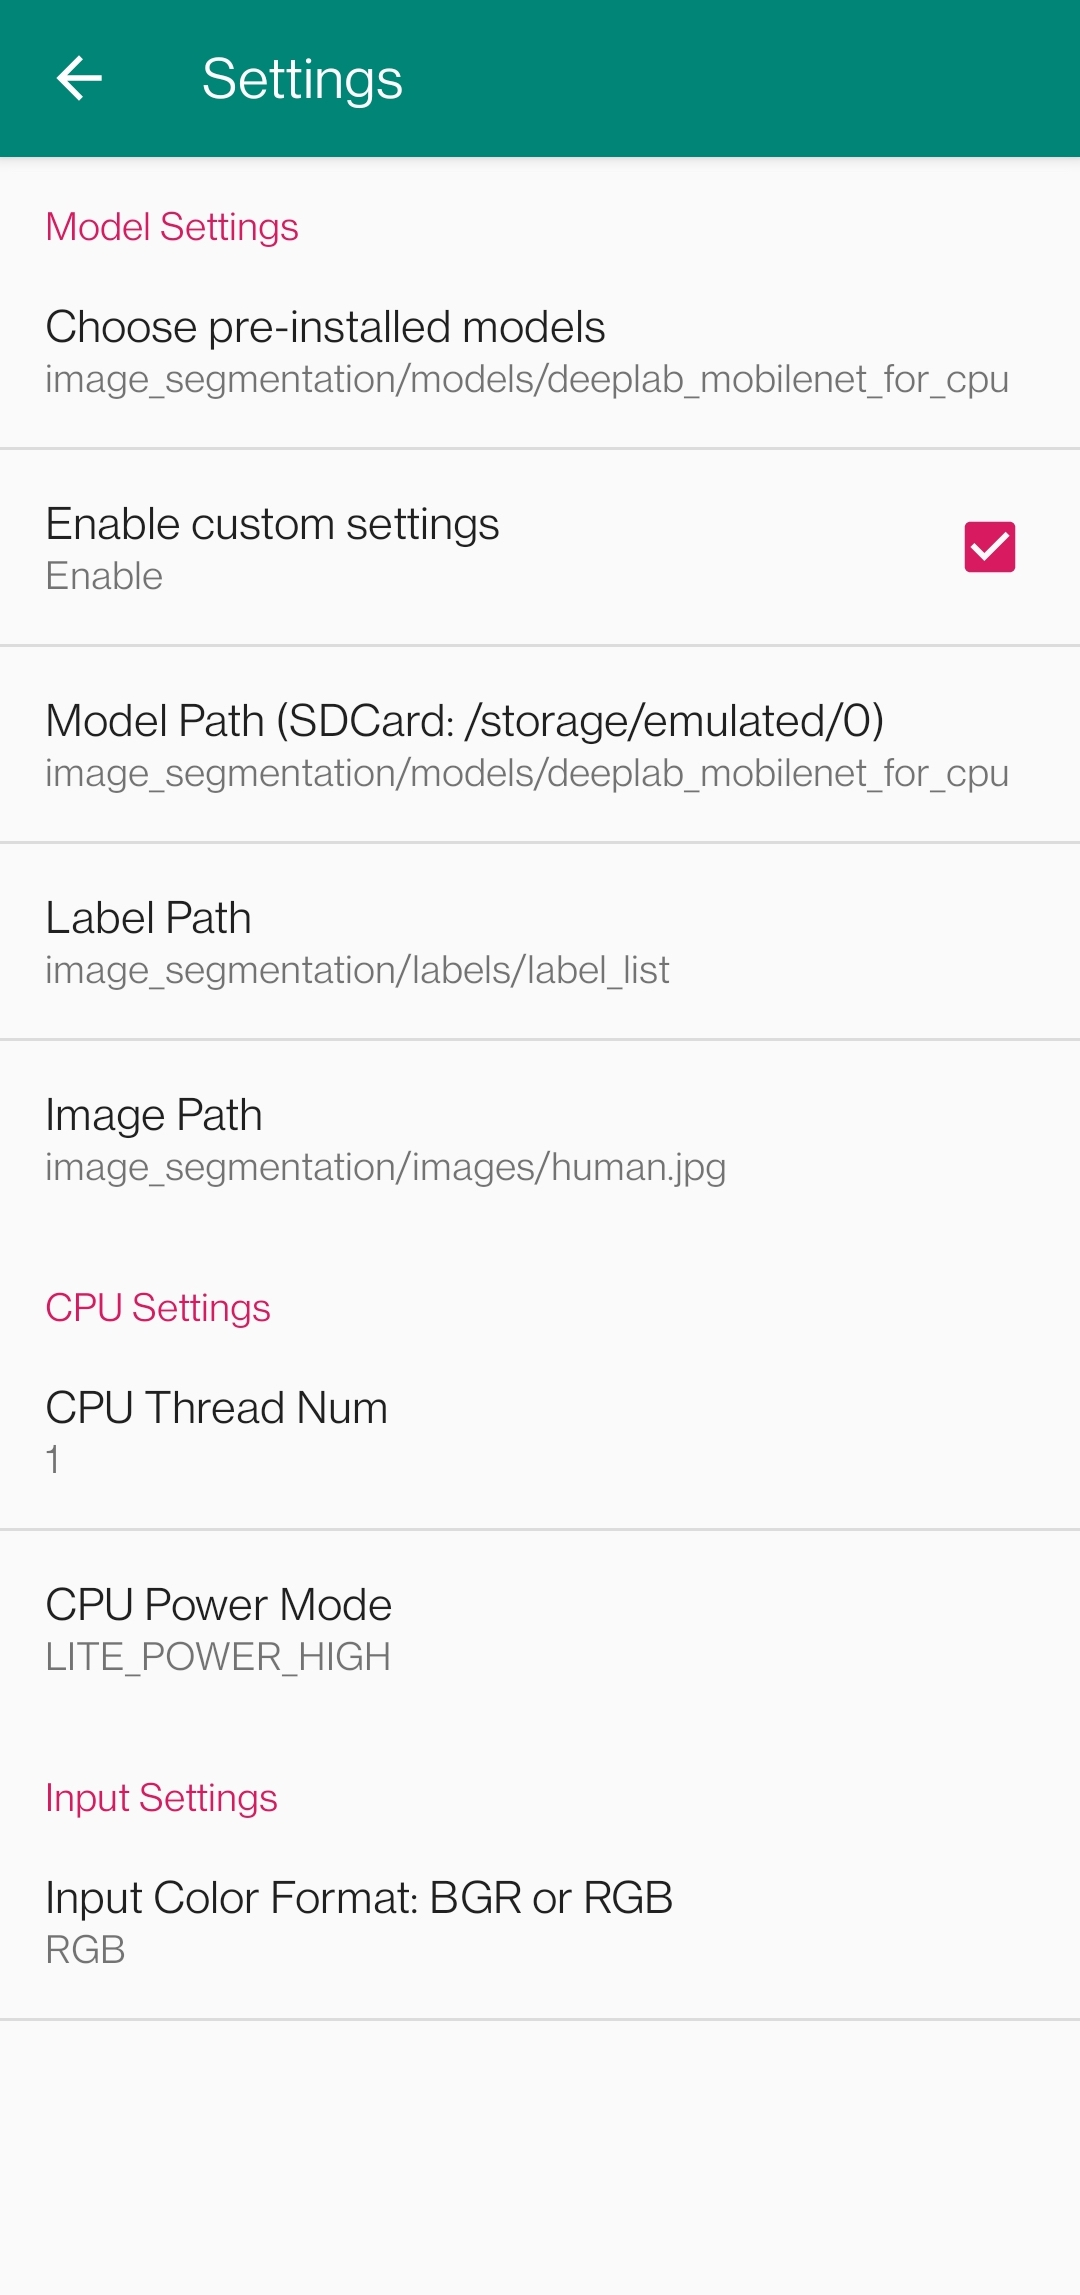
\includegraphics[width=1\textwidth]{figures/settings.jpg}
        \caption{The Whole Settings Page}\label{settings}
    \end{subfigure}
    \begin{subfigure}[t]{0.4\linewidth}
        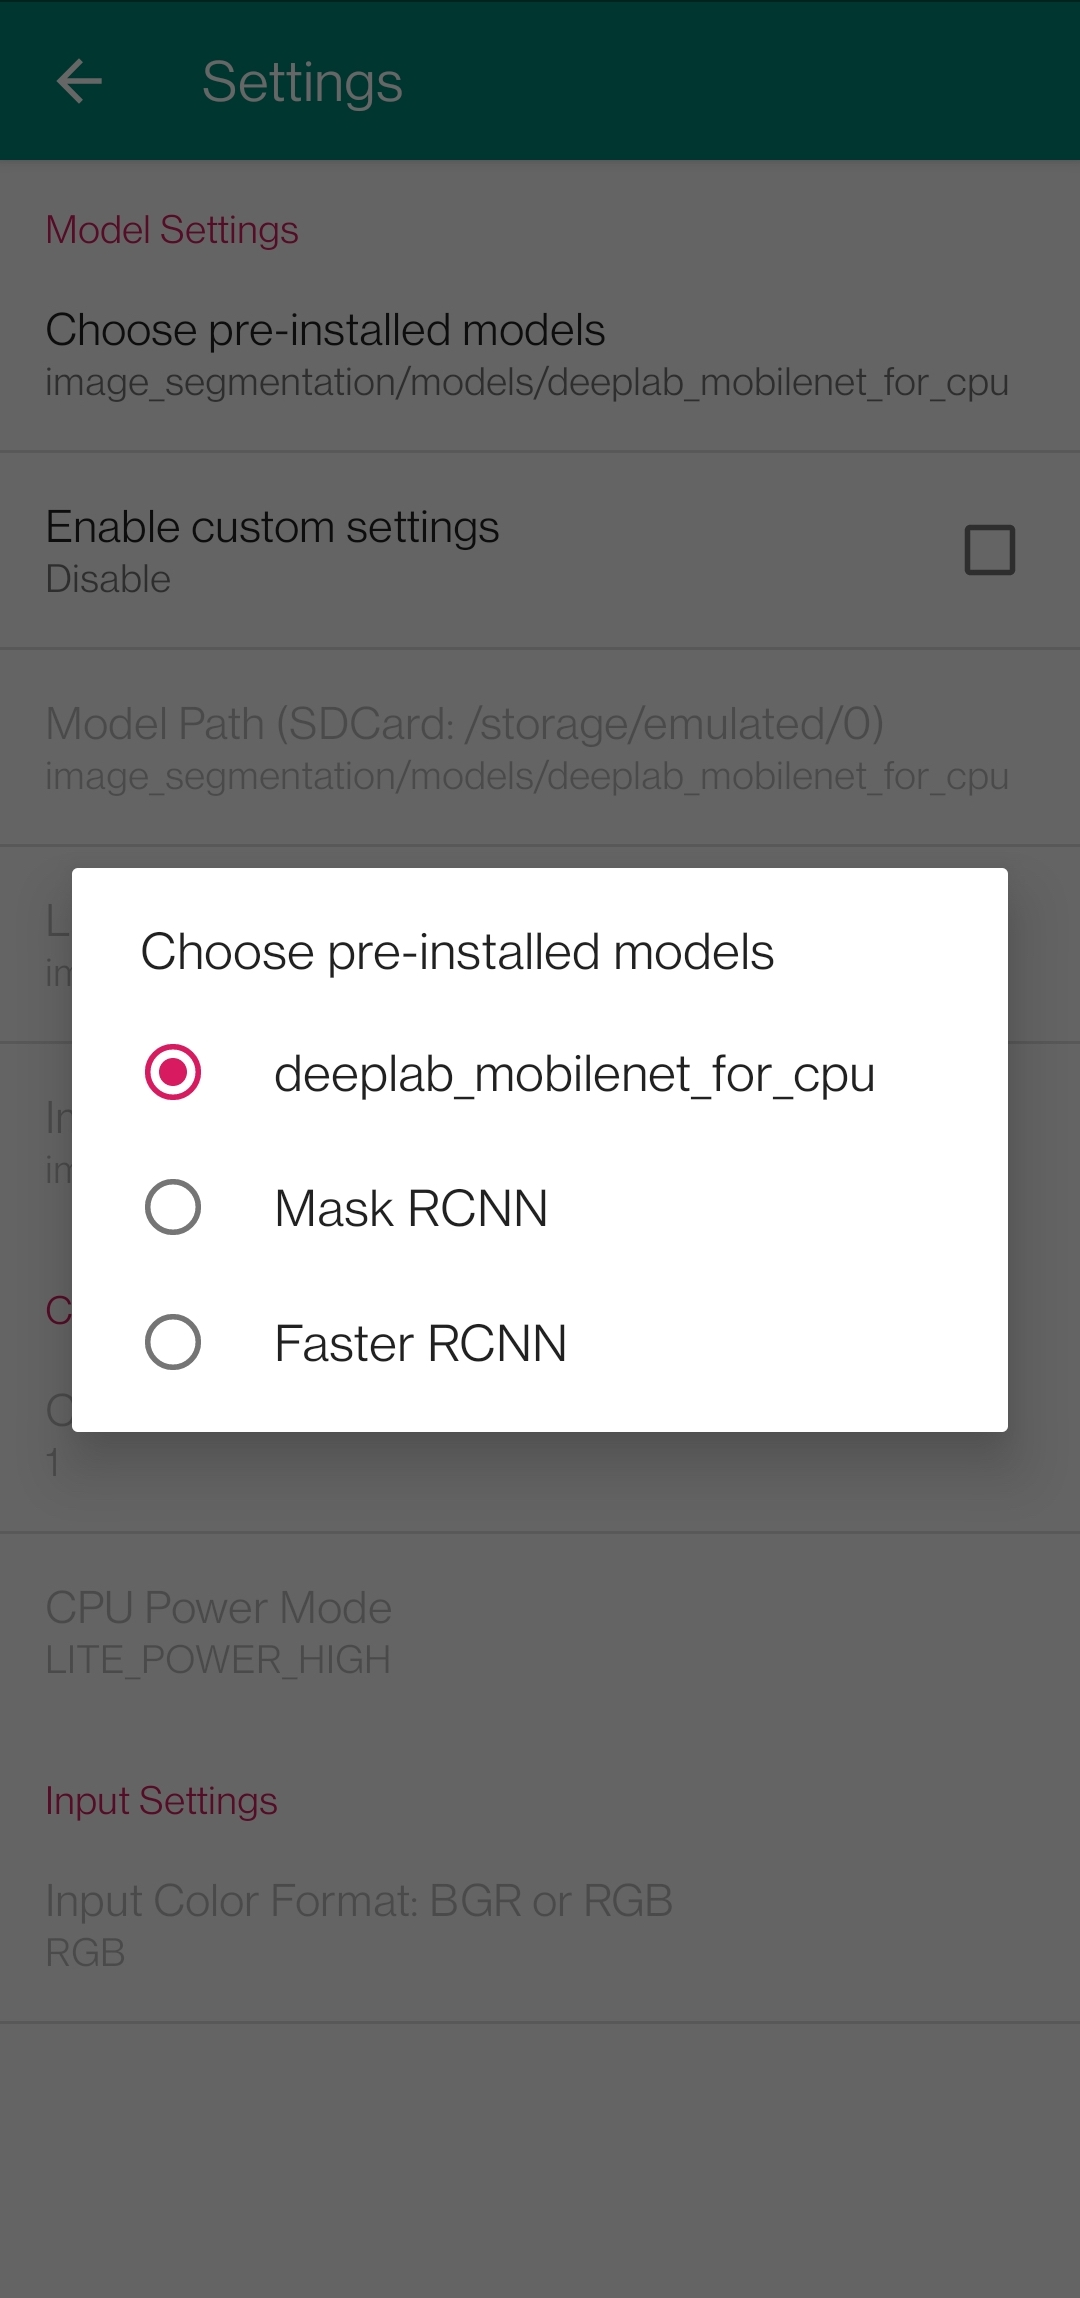
\includegraphics[width=1\textwidth]{figures/type.jpg}
        \caption{Selection Setting about Pre-installed Models}\label{type}
    \end{subfigure}
    \caption{Settings Pages}\label{result1}
\end{figure}

\begin{figure}[htbp]
    \centering
    \begin{subfigure}[t]{0.3\linewidth}
        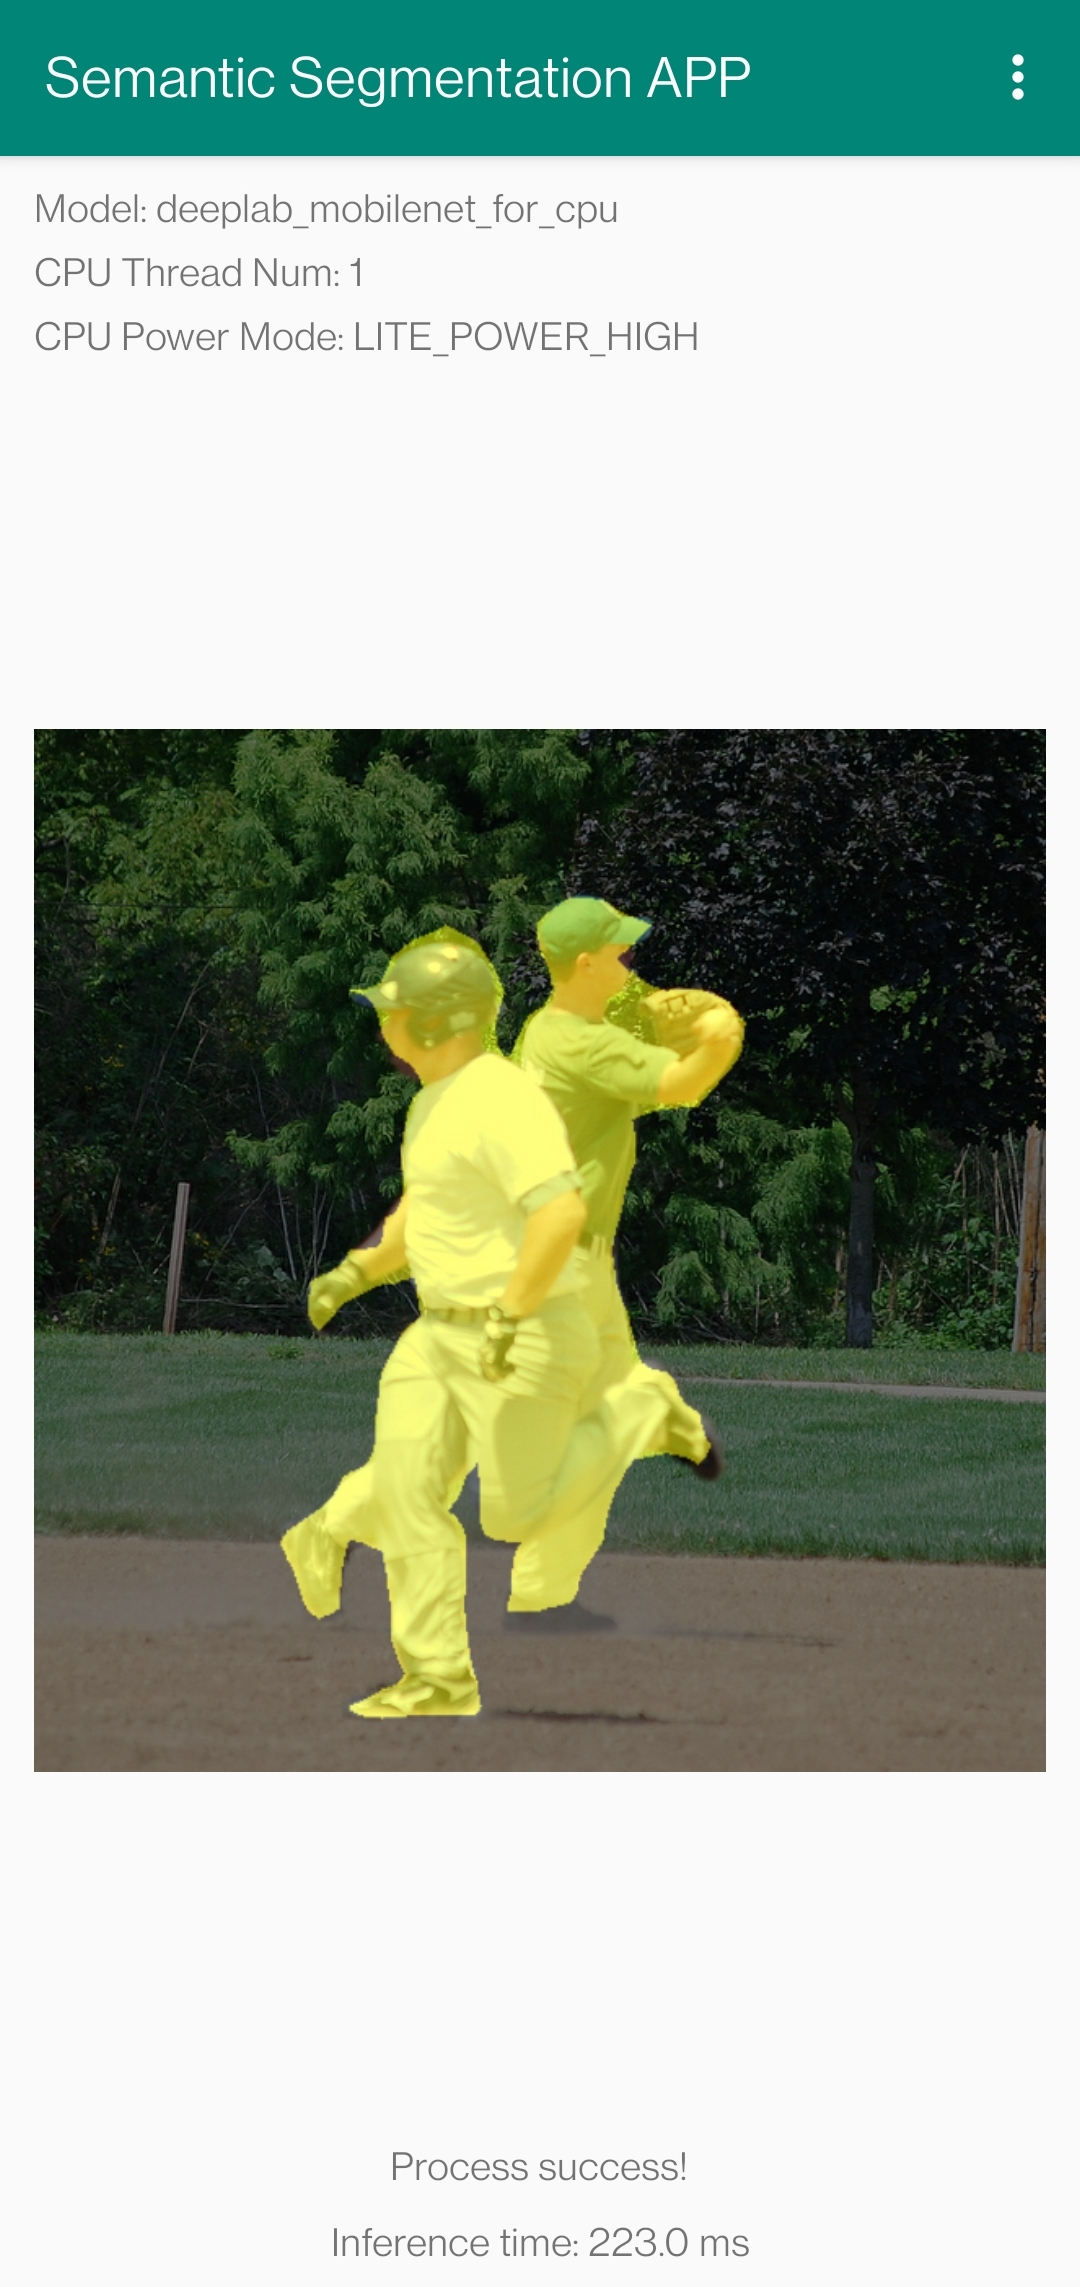
\includegraphics[width=1\textwidth]{figures/paddleresult.jpg}
        \caption{Segmentation Result of Paddle Lite}\label{resultpaddle}
    \end{subfigure}
    \begin{subfigure}[t]{0.3\linewidth}
        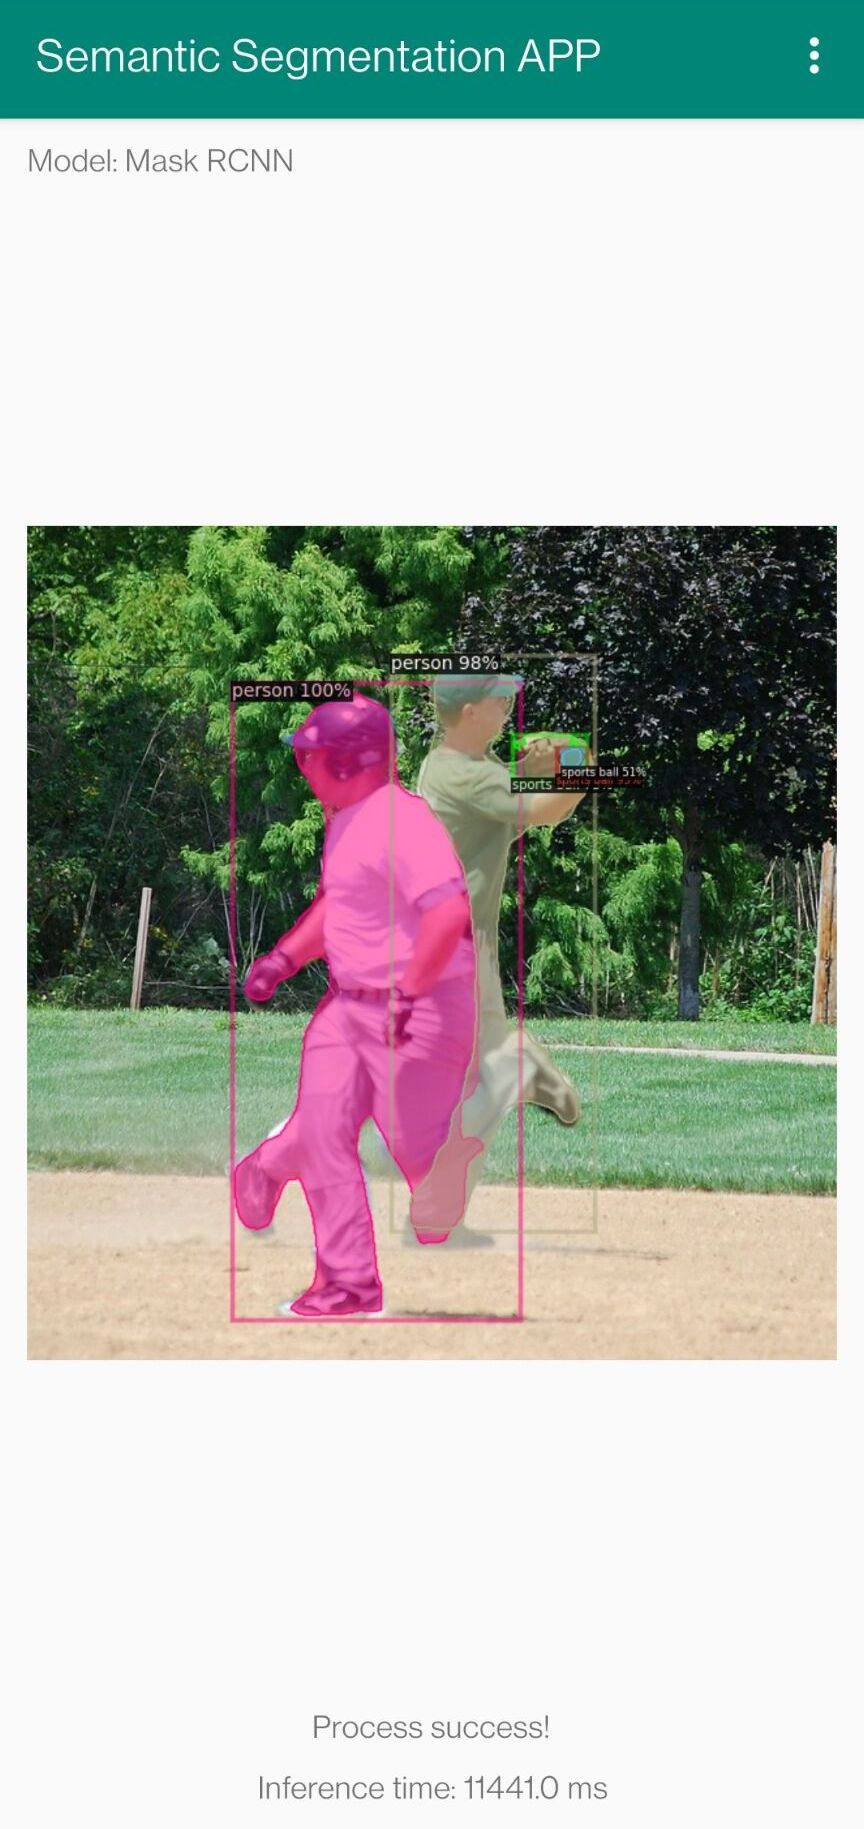
\includegraphics[width=1\textwidth]{figures/maskresult.jpg}
        \caption{Segmentation Result of Mask RCNN}\label{resultmaskrcnn}
    \end{subfigure}
    \begin{subfigure}[t]{0.3\linewidth}
        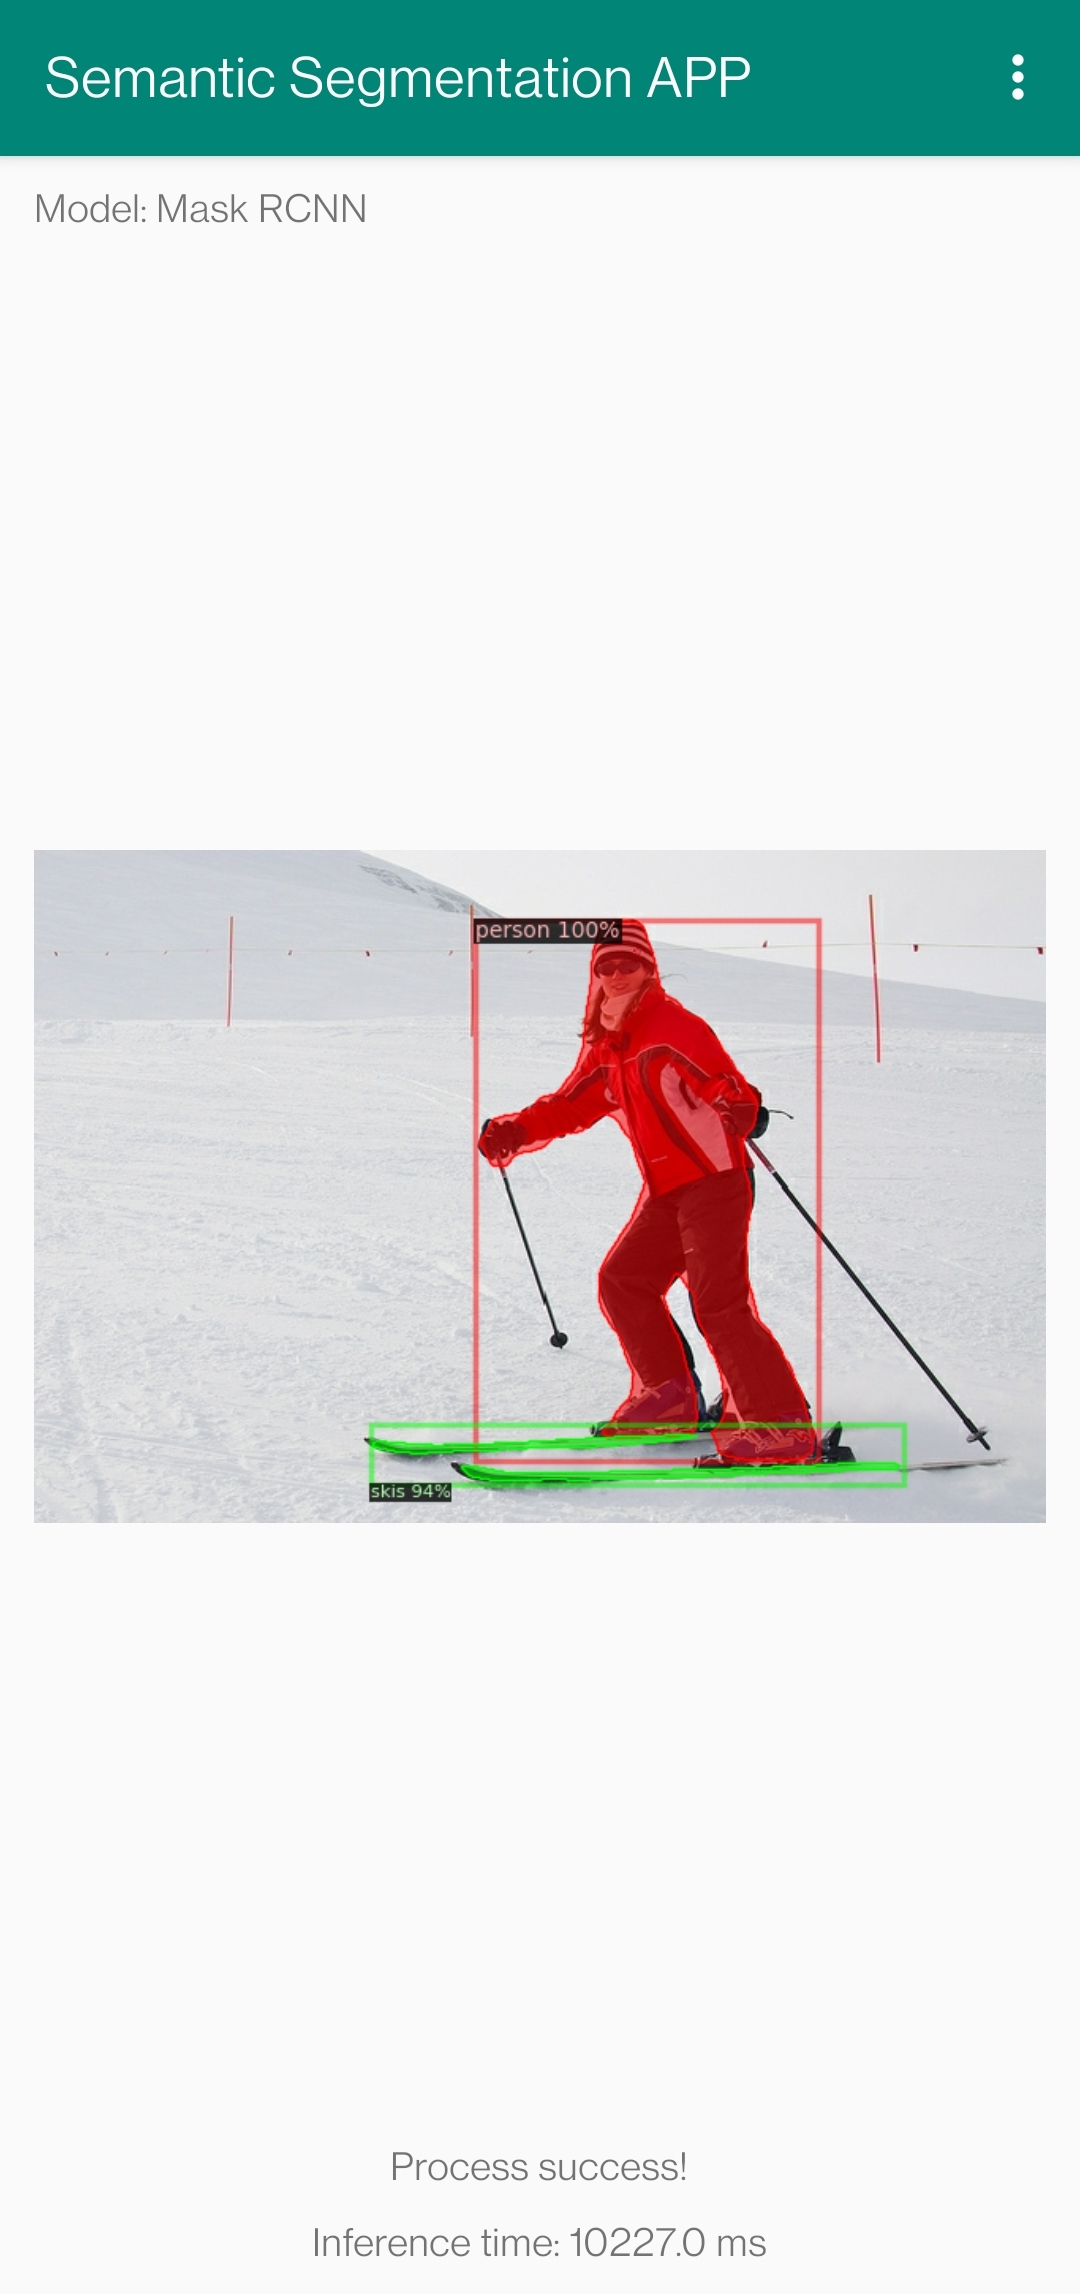
\includegraphics[width=1\textwidth]{figures/ski.jpg}
        \caption{Segmentation Result of Mask RCNN}\label{resultskimaskrcnn}
    \end{subfigure}
    \caption{Result With Different Model and Images}\label{result2}
\end{figure}

%该部分选取了APP的设置页面和分割结果予以展示。设置页面提供了对于模型的选项,用户可以在设置页面里选择模型的路径,图像的路径和通道顺序等等。对于结果来说,可以看到对于物体及其边界的识别的效果较好,而对于实力分割中同类的存在重叠物体的边界识别还存在问题。但是对于单独物体的识别和分割的效果较好,达到了预期。

This part selects the settings page of the APP and the segmentation results to display. The settings page provides options for the model, the user can choose the path of the model, the path of the image and the channel order, etc. on the settings page. For the results, it can be seen that the recognition of objects and their boundaries is better, but there are still problems in the recognition of the boundaries of overlapping objects of the same kind in strength segmentation. However, the effect of recognition and segmentation of individual objects is better, which has reached the expectation.

%其中可以看到在使用非预移植模型时,处理所需的时间较长。其中对于尺寸较大的图片,80%左右的时间用于数据传输,10%左右的时间用于加载模型,10%左右的时间用于分割。对于尺寸较小的图像也仅有50%的时间是真正用于模型的运行。模型运行的效率约为$2s/Obj$

It can be seen that the processing time is longer when using the non-preported model. Among them, for large-sized images, about 80\% of the time is used for data transmission, about 10\% of the time is used to load the model, and about 10\% of the time is used for segmentation. For smaller images, only 50\% of the time is used for running the model. The model runs with an efficiency of about $2s/Obj$.

%总的来说,本论文在Faster R-CNN和Mask R-CNN和FaPN模型的训练结果上取得了不逊于原论文的结果,并部署在了服务器端。在与移动端模型相比较时,在模型加载速度和效率上略逊于移动端模型,但在分割效果,特别是对于小物体和物体边缘的分割上取得了显著优势。

In general, this paper achieves comparable results to the original paper on the training results of Faster R-CNN, Mask R-CNN, and FaPN models, which are deployed on the server-side. When compared with the mobile-end model, the model loading speed and efficiency are slightly inferior to the mobile-end model, but it has achieved significant advantages in segmentation effect, especially for the segmentation of small objects and object edges.

\subsection{Environment}

\begin{itemize}
    \item \textbf{Model training environment: }
    
    1 Intel(R) Xeon(R) Gold 6226 CPU @ 2.70GHz

    2 NVIDIA GeForce RTX 2080Ti graphics cards

    Torch version: 1.7.1+cu101

    Python 3.6.9
    \item \textbf{Model running environment: }

    1 Intel(R) Xeon(R) Platinum 8255C CPU @ 2.50GHz

    No GPU

    Torch version: 1.8.0+cpu

    Python 3.8.10
    \item \textbf{Training Parameters: }

    Iterations: Mask R-CNN \& Faster R-CNN with $1 * 10^4\  \&\  2 * 10^4$

    Learning Rate $0.0002\  \&\  0.0001$, better result chosen

    Other parameters are consistent with the paper FaPN

    \item \textbf{Other Tools Used: }
    
    \href{https://github.com/HarisIqbal88/PlotNeuralNet}{PlotNeuralNet} \cite{plotNeuralNet}

    \href{https://github.com/facebookresearch/detectron2}{detectron2} \cite{wu2019detectron2}

    \href{https://github.com/iydon/sustechthesis}{sustechthesis} \cite{sustechthesis}


\end{itemize}


%true positive(TP)
%false positive(FP)
%true negative(TN)
%false negative(FN)
%mIOU=TP/(FP+FN+TP),i表示真实值,j表示预测值,pij表示将i预测为j

% \begin{figure}[htb]
%     \centering
%     \includegraphics[width=.5\textwidth]{example-image-a}
%     \caption{Test image}\label{F:test-a}
%     % 图片的标题应该在下方
% \end{figure}

% \begin{figure}[htb]
%     \centering
%     \begin{subfigure}[t]{.45\linewidth}
%         \centering
%         \includegraphics[width=1\textwidth]{example-image-a}
%         \caption{子图-自带测试图片---Test image}\label{F:test-b-sub-a}
%     \end{subfigure}
%     \begin{subfigure}[t]{.45\linewidth}
%         \centering
%         \includegraphics[width=1\textwidth]{example-image-a}
%         \caption{子图-自带测试图片---Test image}\label{F:test-b-sub-b}
%     \end{subfigure}
%     \caption{自带测试图片---Test image}\label{F:test-b}
% \end{figure}
\clearpage